\begin{example}
    For $n = 0$:
    \[f(x) = f(c) + f'(\xi_x)(x - c)\]
    Choose $c = a$, $x = b$:
    \[
        f(b) = f(a) + f'(\xi_x)(b - a) \Longleftrightarrow
        f'(\xi_x) = \frac{f(b) - f(a)}{b - a}
    \]
    This is the mean value theorem!
    \begin{figure*}[h]
        \caption{Mean value theorem illustration}
        \centering
        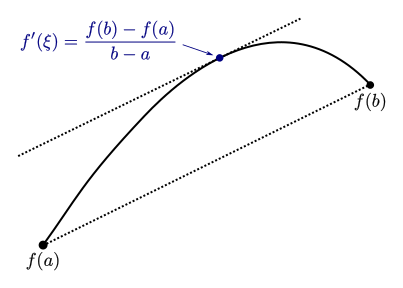
\includegraphics[width=0.5\textwidth]{mean_value_theorem}
    \end{figure*}
\end{example}

\begin{definition}
    We say that the Taylor series \textit{represents} the function $f$ at $x$
    if the Taylor series converges at that point, i.e. the remainder 
    tends to zero as $n \to \infty$.
\end{definition}

\begin{example}[1]
Back to $e^x$: $f(x) = e^x$, $c = 0$, $\xi_x$ is between $c$ and $x$.
\[
    e^x = \sum_{k=0}^n \frac{x^k}{k!} + \frac{e^{\xi_x}}{(n + 1)!} x^{n + 1}
\]

For any $x \in \mathbb{R}$ we find $s \in \mathbb{R}^{+}_{0}$ ($\mathbb{R}^{+}_{0}$ are
all real, positive numbers including 0)
so that $\abs{x} \le s$, and $\abs{\xi_x} \le s$ because $\xi_x$ is between $c$ and $x$.

\begin{figure*}[h]
    \centering
    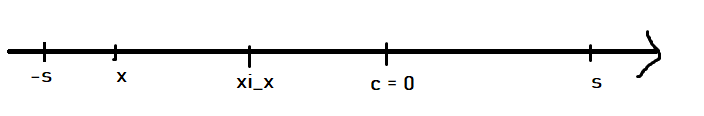
\includegraphics[width=0.5\textwidth]{some_axis}
\end{figure*}

\pagebreak
Because $e^x$ is monotone increasing, we have $e^{\xi_x} \le e^s$, thus

\begin{align*}
    \lim_{n \to \infty} \abs{\frac{e^{\xi^x}}{(n+1)!} x^{n + 1}} \le
    \lim_{n \to \infty} \abs{\frac{e^s}{(n + 1)!}} s^{n + 1} = 
    e^s \lim_{n \to \infty} \frac{s^{n + 1}}{(n + 1)!} = 0
\end{align*}

Because $(n + 1)!$ will grow faster than any power of
$s \implies \lim_{n \to \infty} \abs{\frac{e^{\xi_x}}{(n + 1)!} x^{n + 1}} = 0$.

Thus $e^x$ is \textit{represented} by its Taylor series.
\end{example}

\begin{example}[2]
    \begin{align*}
        &
        f(x) = \log(1 + x),\ c = 0
        \\&
        f'(x) = \frac{1}{1+x} = (1 + x)^{-1}
        \\&
        f''(x) = -(1 + x)^{-2}
        \\&
        f'''(x) = +2(1 + x)^{-3}
        \\&
        f^{(k)}(x) = (-1)^{k + 1} (k - 1)! \frac{1}{(1 + x)^k}
    \end{align*}
\end{example}

So $f^{(k)}(0) = (-1)^{k - 1} (k - 1)!$ for $k \ge 1$, 
$f(0) = \log(1) = 0$.

Taylor series: 
\begin{align*}
    &
    f(x) = \sum_{k = 1}^n \frac{(-1)^{k - 1}}{k} x^k +
    \frac{(-1)^k}{n + 1} \frac{1}{(1 + \xi_x)^{n + 1}} \cdot x^{n + 1}
    \quad \Bigl(\frac{n!}{(n + 1)!} = \frac{1}{n + 1}\Bigr)
    \\&
    E_n(x) = \frac{(-1)^k}{n + 1} \frac{1}{(1 + \xi_x)^{n + 1}} \cdot x^{n + 1}
    \text{ --- the remainder}
\end{align*}
Question: for which $x$ does $\lim_{n \to \infty} E_n(x) = 0$?
\[
    \lim_{n \to \infty} E_n(x) =
    \lim_{n \to \infty} \frac{(-1)^n}{n + 1} \Bigl(\frac{x}{\xi_x + 1}\Bigr)^{n + 1}
    \text{ for } \xi_x \in (c, x)\ (c = 0)
\]
Such a limit converges to 0, if the fraction is less than 1.
\[
    0 < \frac{x}{\xi_x + 1} < 1 \Longleftrightarrow x < \xi_x + 1 \Longleftrightarrow
    x - \xi_x < 1 \text{ with } \xi_x \in (0, x) \Longleftrightarrow
    x \le 1
\]
\begin{consequence}
    $\lim_{n \to \infty} E_n(x) = 0$ if $0 < x \le 1$.
    This means that the Taylor series represents $\log(x + 1)$ for $x \in [0, 1]$.
    We can extend this to show $x \in (-1, 1]$.
\end{consequence}

\begin{example}[3]
    Let's compute $\cos(0.1)$. Let's approximate it with Taylor series with $c = 0$ (around zero).
    \[
        \cos(x) = 1 - \frac{x^2}{2} + \frac{x^4}{4!} - \frac{x^6}{6!} \pm \dots
        + \mathrm{remainder}
    \]
\end{example}
\begin{consequence}
    \[
        \abs{\cos(x) - \sum_{k=0}^n (-1)^k \frac{x^{2k}}{(2k!)}} =
        \abs{(-1)^{n + 1} \cos(\xi_x) \frac{x^{2(n + 1)}}{\bigl(2(n + 1)\bigr)!}} \le
        \frac{0.1^{2(n + 1)}}{2(n + 1)!} \underset{n \to \infty}{\longrightarrow} 0
    \]
\end{consequence}

\begin{center}
    \begin{tabular}{c | c | c}
        $n$ & Taylor polynomial & $\abs{error} \le$\\
        \hline
        0 & 1 & $\frac{(0.1)^2}{2} = 0.0005$\\
        1 & 0.995 & $\frac{0.0001}{24}$\\
        2 & 0.99500416 & $\frac{0.000001}{6!}$
    \end{tabular}
\end{center}

Error depends on choice of $\abs{x - c}$ and $n$.

\begin{example}[4]
    Compute $\log(2)$ using $f(x) = \log(x + 1)$
    \[
        \log(2) = 1 - \frac{1}{2} + \frac{1}{3} - \frac{1}{4} + \frac{1}{5} - \frac{1}{6} + \dots
    \]
    Keeping 8 terms (until $n = 8$) we get
    $\log(2) \approx 0.63452$, the actual solution is $\log(2) = 0.693147$. Not so accurate. Can we improve?

    We can use Taylor series of $\log\bigl(\frac{1 + x}{1 - x}\bigr)$ instead, 
    since $\log\bigl(\frac{1 + x}{1 - x}\bigr) = \log(1 + x) - \log(1 - x)$.
    We choose $x = \frac{1}{3}$ instead of $x = 1$.
    Since $x$ is closer to zero, both of the logarithms converge quicker.
    \[
        \biggl(\log\Bigl(\frac{1 + 1/3}{1 - 1/3}\Bigr) = \log(2) \biggr)
    \]
    We then get
    \[
        \log(2) = 2 \cdot \Bigl(\frac{1}{3} + \frac{1}{3^3 \cdot 5} + \dots\Bigr)
    \]
    We only need 4 terms to get
    $\log{2} \approx 0.69313$.
\end{example}

\begin{theorem}[Reformulation of Taylor's theorem]
    $f \in \mathrm{C}^{n + 1}([a, b])$. We change $c$ to $x$ and the old $x$
    to $x + h$ from previous version $\implies$
    get for $x,\ x + h \in [a, b]$:
    \[
        f(x + h) = \sum_{k = 0}^n \frac{f^{(k)}(x)}{k!} h^k + 
        \frac{f^{(n + 1)}(\xi_x)}{(n + 1)!} h^{n + 1}
        \text{ where } \xi_x \in (x, x + h),\ h > 0
    \]

    We can write error term as 
    \[
        f(x + h) - \sum_{k=0}^n \frac{f^{(k)}(x)}{k!} h^k = \mathcal{O}(h^{n + 1})
    \]
\end{theorem}
\begin{remark}
    Let's recall what the $\mathcal{O}$-notation means.
    $a(h) = \mathcal{O}\bigl(b(h)\bigr)$ if $\exists c > 0$
    such that $\frac{a(j)}{b(j)} \le c$ as $h \to 0$.
    So, for $n = 1$ the error decreases with $h^2$ (quadratic convergence).\\
    $n = 2$: error decreases cubically, i.e. $h^3$, etc.
\end{remark}